\section{Methods}

\subsection{Reliability and availability of data centers}

\subsubsection{Introduction}\label{subsubsection: introduction - dependability}

\definition{Dependability} is a \textbf{comprehensive measure} of how much we can \textbf{trust a system} to perform its expected function correctly and consistently over time.

\highspace
Dependability is not a single property but a \textbf{composite of multiple interrelated concerns}, some more related to system correctness (reliability, availability), others more to protection (safety, security). In large-scale systems like datacenters, \textbf{dependability is not optimal}, it is integral to Service Level Agreement (SLAs)\footnote{%
    A \definition{Service Level Agreement (SLA)} is a contract between a service provider and a customer that defines the expected level of service. It typically includes metrics like availability, performance, and response times, along with remedies if the provider fails to meet those standards.
}, customer trust, and legal compliance (e.g., data protection laws)\footnote{%
    \textbf{Legal compliance} in data protection laws ensures that organizations handle personal data responsibly and in accordance with regulations. In the EU, the \emph{General Data Protection Regulation (GDPR)} is the primary framework, setting strict rules on data collection, processing, and storage. Globally, different countries have their own laws, such as the \emph{California Consumer Privacy Act (CCPA)} in the U.S., and similar regulations emerging worldwide.
}.

\highspace
\begin{flushleft}
    \textcolor{Green3}{\faIcon{book} \textbf{Core Attributes of Dependability}}
\end{flushleft}
\begin{table}[!htp]
    \centering
    \begin{adjustbox}{width={\textwidth},totalheight={\textheight},keepaspectratio}
        \begin{tabular}{@{} l p{13em} p{17em} @{}}
            \toprule
            \textbf{Attribute} & \textbf{Meaning} & \textbf{Analogy / Data Center View} \\
            \midrule
            \textbf{Reliability}        & Continuity of correct service         & A web server not crashing or corrupting data for long periods. \\ [.5em]
            \textbf{Availability}       & Readiness for correct service         & Can the system serve requests \emph{right now}? \\ [.5em]
            \textbf{Maintainability}    & Ability for easy maintenance          & Hot-swappable disks, modular servers. \\ [.5em]
            \textbf{Safety}             & Absence of catastrophic consequences  & E.g., fail-safes in a power system to avoid fire/electrical hazard. \\ [.5em]
            \textbf{Security}           & Confidentiality and integrity of data & Access control, data encryption, intrusion prevention. \\
            \bottomrule
        \end{tabular}
    \end{adjustbox}
\end{table}

\begin{examplebox}[: Cloud Service Provider]
    Image Google Cloud or AWS:
    \begin{itemize}
        \item \textbf{Reliability}: Our VMs shouldn't crash without reason.
        \item \textbf{Availability}: We must access our cloud database anytime.
        \item \textbf{Maintainability}: They update the hypervisor with zero downtime.
        \item \textbf{Safety}: If a cooling system fails, automatic shutdown prevents hardware fire.
        \item \textbf{Security}: Data encryption at rest and in transit, isolation across tenants.
    \end{itemize}
\end{examplebox}

\highspace
\begin{flushleft}
    \textcolor{Green3}{\faIcon{question-circle} \textbf{Do we really need to care about Dependability?}}
\end{flushleft}
First, we'll explore intuition. Even when a system is \emph{well-designed}, passes \emph{functional verification}, meets \emph{performance and energy constraints}, it can still \textbf{fail}! Why? Because real-world conditions and \textbf{non-functional factors} can break even perfectly specified systems.

\highspace
So dependability is \underline{necessary} because \hl{\textbf{failures are inevitable}}. They stem from \textbf{multiple layers of system stack}, including:

\begin{table}[!htp]
    \centering
    \begin{tabular}{@{} l | l @{}}
        \toprule
        \textbf{Source} & \textbf{Example} \\
        \midrule
        \textbf{Hardware aging}             & Transistor degradation, wear-out mechanisms.  \\ [.5em]
        \textbf{Manufacturing defects}      & Process variation, cosmic rays.               \\ [.5em]
        \textbf{Design flaws}               & Logic errors, incorrect specifications.       \\ [.5em]
        \textbf{Software bugs}              & Memory leaks, race conditions, kernel panics. \\ [.5em]
        \textbf{System misconfiguration}    & Wrong firewall rule, VM setting.              \\ [.5em]
        \textbf{External disturbances}      & Electromagnetic interference, overheating.    \\ [.5em]
        \textbf{Human errors}               & Mistakes by admins, developers.               \\ [.5em]
        \textbf{Malicious attacks}          & DoS, ransomware, data exfiltration.           \\
        \bottomrule
    \end{tabular}
\end{table}

\noindent
Even a tiny misbehavior in one layer can cascade through the entire system.

\highspace
\begin{flushleft}
    \textcolor{Red2}{\faIcon{exclamation-triangle} \textbf{Consequences of Undependability}}
\end{flushleft}
Let's categorize \textbf{why lack of dependability is dangerous}, especially in data centers:
\begin{enumerate}
    \item \important{High Economic Cost}: Downtime may cause lost transactions, SLA violations, brand damage.
    \item \important{Information Loss}: Permanent deletion or corruption of critical data (e.g., backups overwritten, logs lost).
    \item \important{Cascade Failures}: One component failure affects dependent services (e.g., cloud outages).
    \item \important{User Distrust}: If users don't trust the service, they abandon it.
    \item \important{Security \& Safety Hazards}: leaked credentials, incorrect data processing and in physical systems, risk to human life (think healthcare or industrial systems).
\end{enumerate}

\highspace
\begin{flushleft}
    \textcolor{Green3}{\faIcon{question-circle} \textbf{When to Think About Dependability?}}
\end{flushleft}
Short answer: \textbf{Always}. Dependability is \textbf{not an optional}, it must be \textbf{considered} throughout the \textbf{entire system lifecycle}: \emph{design-time}, \emph{deployment}, \emph{run-time}, and even \emph{decommissioning}. We think about dependability:
\begin{itemize}
    \item At \important{Design-Time}, the main goal is to \textbf{prevent as many failures as possible before the system is deployed}. This is when we:
    \begin{itemize}
        \item \textbf{Analyze}: Model the system and predict how it behaves under faults.
        \item \textbf{Measure}: Evaluate expected MTTF, availability, error rates.
        \item \textbf{Optimize}: Adjust design to improve weak points (e.g., redundancy, replication).
        \item \textbf{Verify}: Perform fault-injection, static analysis, formal verification.
    \end{itemize}
    \item At \important{Run-Time}, no matter how good our design is, \hl{failures will still happen} in the field. So \textbf{we must}:
    \begin{itemize}
        \item \hl{Detect}: \textbf{Monitor system} state to spot abnormal behavior.
        \item \hl{Diagnose}: \textbf{Understand} root \textbf{causes} (e.g., logs, telemetry).
        \item \hl{React}: \textbf{Automatically correct} or \textbf{isolate} the problem.
    \end{itemize}
    For example rebooting a crashed VM, replacing a failed disk in a RAID array or routing traffic away from an unhealthy load balancer.
\end{itemize}

\highspace
\begin{flushleft}
    \textcolor{Green3}{\faIcon{balance-scale} \textbf{Why Distinguish Development-Time vs Operation-Time Failures?}}
\end{flushleft}
These two types of failures have completely different roots, so we must use different strategies to handle them. 
\begin{itemize}
    \item \definition{Development-Time Failures}. These are \textbf{errors that are introduced during system creation}, in the design, coding or configuration phase.

    \begin{itemize}
        \item[\textcolor{Green3}{\faIcon{tools}}] \textcolor{Green3}{\textbf{Examples}}
        \begin{itemize}
            \item A bug in the file system code that causes data corruption.
            \item A wrong assumption in system specifications.
            \item An incorrect server configuration (e.g., firewall blocking valid ports).
            \item A logic error in redundancy management (e.g., mirrored disk not syncing).
        \end{itemize}
        \item[\textcolor{Green3}{\faIcon{check}}] \textcolor{Green3}{\textbf{Solutions}}
        \begin{itemize}
            \item These \textbf{should be avoided} before deployment.
            \item They're addressed using:
            \begin{itemize}
                \item \textbf{Testing} (unit, integration, fault-injection)
                \item \textbf{Verification} (formal methods, code reviews)
                \item \textbf{Validation} (does it meet real-world expectations?)
            \end{itemize}
        \end{itemize}
        \item[\textcolor{Red2}{\faIcon{exclamation-triangle}}] \hl{If a system fails} due to a development-time error, it means there was something \textbf{wrong in how it was built}.
    \end{itemize}
    

    \newpage


    \item \definition{Operation-Time Failures}. These are \textbf{failures that happen while the system is running}, even if the system was perfectly designed.
    
    \begin{itemize}
        \item[\textcolor{Green3}{\faIcon{tools}}] \textcolor{Green3}{\textbf{Examples}}
        \begin{itemize}
            \item A hard disk physically fails after 3 years.
            \item A memory bit flips due to cosmic radiation (soft error).
            \item The power supply overheats due to dust.
            \item A data center operator accidentally disconnects a cable.
            \item A hacker exploits an unknown vulnerability.
        \end{itemize}
        \item[\textcolor{Green3}{\faIcon{check}}] \textcolor{Green3}{\textbf{Solutions}}
        \begin{itemize}
            \item These \textbf{cannot be entirely avoided}, because hardware ages, users make mistakes, environments are unpredictable.
            \item They \textbf{must be handled at runtime} with:
            \begin{itemize}
                \item \textbf{Monitoring}
                \item \textbf{Redundancy / Fault tolerance}
                \item \textbf{Error correction \& self-repair}
            \end{itemize}
        \end{itemize}
        \item[\textcolor{Red2}{\faIcon{exclamation-triangle}}] \hl{If a system fails} at runtime, it's not necessarily badly designed, \textbf{reality is imperfect}, and we need to plan for that.
    \end{itemize}
\end{itemize}

\highspace
\begin{flushleft}
    \textcolor{Green3}{\faIcon{question-circle} \textbf{Where to Apply Dependability?}}
\end{flushleft}
Originally, dependability was essential only in a few extreme environments, systems where a failure could endanger lives, waste millions or billions, be unacceptable by definition (space, nuclear, aviation). The \hl{types of Critical Systems}:
\begin{itemize}
    \item \definition{Mission-Critical Systems}. The \textbf{mission} is \textbf{not completed if a failure occurs}. Some examples are satellites (loss $=$ mission failure), unmanned vehicles (e.g., drones, crash $=$ loss of platform and data). \textbf{Dependability ensures the system fulfills its intended goal}.

    \item \definition{Safety-Critical Systems}. If a failure occurs, human life is at risk. Some examples are aircraft control (system crash $=$ airplane crash), nuclear plant controls (meltdown). Here, the \textbf{cost of failure is catastrophic}.
\end{itemize}
\textbf{Dependability today is no longer limited} to space and nuclear systems. Now it's \textbf{central to computing infrastructures}, including data centers, cloud platforms, edge devices, etc. Why? Because a failure today in these systems can disrupt global services (e.g., Gmail outage), leak personal data, etc.

\newpage

\begin{flushleft}
    \textcolor{Green3}{\faIcon{question-circle} \textbf{How to Provide Dependability?}}
\end{flushleft}
Provide Dependability means designing our system (hardware and software) in a way that it \textbf{keeps working}, even when \textbf{things go wrong}, or at least, it fails in a \textbf{safe and recoverable way}. There are \textbf{two main strategies} to achieve this:
\begin{enumerate}
    \item \definition{Failure Avoidance} (try not to fail). This approach is like saying: ``\emph{let me build the system so well that it doesn't break}''. For example, use very reliable hardware, run a lot of testing before deploying our software, do quality control in factories to catch early hardware faults, and use formally verified algorithms in critical parts.

    This approach is \textbf{good}, \textbf{but expensive}, and we \textbf{can't predict everything}.

    \begin{examplebox}[: Failure Avoidance Analogy]
        Like buying a car and checking \emph{everything} before leaving the factory: brakes, oil, tires, engine. So it's unlikely to break.
    \end{examplebox}


    \item \definition{Failure Tolerance} (prepare for when it does fail). This approach accepts the fact that something \textbf{will} go wrong. So let us prepare the system to \textbf{detect}, \textbf{contain}, and \textbf{recover} from the problem.

    For example, use RAID for disks, use ECC memory (it can correct small memory errors automatically), monitor servers, and in the cloud, if one data center goes down, reroute to another.

    This is \textbf{essential in data centers}, because with thousands of machines, failures are guaranteed.

    \begin{examplebox}[: Failure Tolerance Analogy]
        Like having a spare tire in our car, a seatbelt, and road assistance. We're ready when things go wrong.
    \end{examplebox}
\end{enumerate}
\textcolor{Green3}{\faIcon{question-circle} \textbf{Where Can We Add Dependability?}} We can ``\emph{add dependability}'' at \textbf{different layers}:
\begin{itemize}
    \item \important{Hardware Level}. Make components themselves very reliable.
    \begin{itemize}[label=\textcolor{Green3}{\faIcon{check}}]
        \item Use robust materials.
        \item Use parts that are known to last a long time.
        \item[\textcolor{Red2}{\faIcon{times}}] Expensive, and maybe slow (old, stable tech).
    \end{itemize}

    \item \important{Architecture/System Design Level}. Make the \textbf{structure of the system} fault-tolerant.
    \begin{itemize}[label=\textcolor{Green3}{\faIcon{check}}]
        \item Duplicate components (e.g., 2 power supplies, RAID).
        \item Create \textbf{clusters}: if one server fails, others can take over
        \item[\textcolor{Red2}{\faIcon{times}}] More machines, more space, higher cost.
    \end{itemize}

    \item \important{Software Level}. Add dependability using \textbf{code}.
    \begin{itemize}[label=\textcolor{Green3}{\faIcon{check}}]
        \item Detect problems: logs, alerts, health checks.
        \item Retry or restart automatically.
        \item Recover from failures (e.g., checkpoint/restart in HPC).
        \item Cheaper and flexible.
        \item[\textcolor{Red2}{\faIcon{times}}] Needs smart design and might slow down performance.
    \end{itemize}
\end{itemize}

\highspace
\begin{flushleft}
    \textcolor{Red2}{\faIcon{exclamation-triangle} \textbf{There ain't no such thing as a free lunch (TANSTAAFL)}}
\end{flushleft}
It is impossible to get something for nothing. We always \textbf{pay} for dependability:

\begin{table}[!htp]
    \centering
    \begin{tabular}{@{} l l @{}}
        \toprule
        We Pay In... & Why? \\
        \midrule
        \textbf{Money}          & Redundant servers, better hardware. \\ [.3em]
        \textbf{Time}           & Development of testing and recovery logic. \\ [.3em]
        \textbf{Performance}    & Extra steps for safety and monitoring. \\
        \bottomrule
    \end{tabular}
\end{table}

\newpage

\subsubsection{Reliability and Availability}

\highspace
\begin{definitionbox}[: Reliability]
    \definition{Reliability} is the probability that a system or component performs its \textbf{required functions}, under \textbf{stated conditions}, for a \textbf{specified period of time} without failure.

    \highspace
    According to IEEE Std 610.12-1990: ``\emph{The ability of a system or component to perform its required functions under stated conditions for a specified period of time.}''
\end{definitionbox}

\highspace
\begin{flushleft}
    \textcolor{Green3}{\faIcon{square-root-alt} \textbf{Mathematical Definition}}
\end{flushleft}
Let $R(t)$ be the reliability function, representing the \textbf{probability that the system has not failed during the time interval} $\left[0, t\right]$:
\begin{equation}
    R(t) = P\left(\text{No failure during } \left[0, t\right]\right) \quad \text{given system was operational at } t = 0    
\end{equation}
\begin{itemize}
    \item $t$ is the time. Reliability always \textbf{depends on the target time window} $t$. For example, a system may be reliable over 10 minutes, but not over 10 hours. In critical systems (like avionics or nuclear control), \textbf{even a short failure} is unacceptable, this makes \textbf{reliability extremely stringent}.
    \item It is a \textbf{non-increasing} function over time.
    \item $R(0) = 1$: at time 0, the system is assumed to be \emph{working}.
    \item $R(t) = 0$ as $t \rightarrow \infty$: over infinite time, failure becomes certain.
\end{itemize}
We can also determine \definition{Unreliability} given the reliability function. Let $Q\left(t\right)$ be the unreliability function:
\begin{equation}
    Q\left(t\right) = 1 - R\left(t\right)
\end{equation}
This express the probability that the system \textbf{has failed} by time $t$.

\highspace
\begin{flushleft}
    \textcolor{Green3}{\faIcon{chart-bar} \textbf{Typical Behavior}}
\end{flushleft}
The failure rate $\lambda\left(t\right)$ may vary over the life of a component:
\begin{itemize}
    \item \textbf{Early stage}: high initial failure due to manufacturing defects.
    \item \textbf{Mid-life}: constant or random failure rate, this is the region of interest in most reliability modeling.
    \item \textbf{End-of-life}: failure rate increases due to wear-out (aging, stress).
\end{itemize}

\newpage

\begin{definitionbox}[: Availability]
    \definition{Availability} is the probability that a system is \textbf{operational and accessible} when it is required to be used.

    It represents how much of the time a system is \textbf{actually up and running}, accounting for both its reliability and its ability to \textbf{recover from failures}.

    \highspace
    According to IEEE Std 610.12-1990: ``\emph{The degree to which a system or component is operational and accessible when required for use.}''
\end{definitionbox}

\noindent
While \textbf{reliability} focuses on \emph{continuous correct operation}, \textbf{availability} emphasizes the \textbf{\emph{readiness for use}} at a given moment, even after failures occur and are repaired.

\highspace
\begin{flushleft}
    \textcolor{Green3}{\faIcon{square-root-alt} \textbf{Mathematical Definition}}
\end{flushleft}
For \textbf{steady-state availability}:
\begin{equation}
    \text{Availability} = \dfrac{\text{Uptime}}{\text{Uptime} + \text{Downtime}}
\end{equation}
Formally, $A\left(t\right)$ is the probability that the system is \textbf{operational} (not failed) at a given time $t$:
\begin{equation}
    A\left(t\right) = P\left(\text{System is working at time } t\right)
\end{equation}
In other words, it's the probability that the system is \textbf{ready for service} at time $t$.
\begin{itemize}
    \item \important{Non-Repairable Systems}. If the system \textbf{cannot be repaired}, then:
    \begin{equation*}
        A(t) = R(t)
    \end{equation*}
    The availability equals the reliability (it will eventually fail and stay\break failed).
    \item \important{Repairable}. For \textbf{repairable systems}:
    \begin{equation*}
        A(t) \geq R(t)
    \end{equation*}
    Because even if the system fails, it may be restored and become available again.
\end{itemize}
We can also determine \definition{Unavailability} given the availability function:
\begin{equation}
    \text{Probability that the system is not operational at time } t = 1 - A(t)
\end{equation}

\newpage

\begin{flushleft}
    \textcolor{Green3}{\faIcon{balance-scale} \textbf{Difference from Reliability}}
\end{flushleft}
\begin{table}[!htp]
    \centering
    \begin{adjustbox}{width={\textwidth},totalheight={\textheight},keepaspectratio}
        \begin{tabular}{@{} l l l @{}}
            \toprule
            \textbf{Concept} & \textbf{Reliability} & \textbf{Availability} \\
            \midrule
            \textbf{Meaning}     & No failure in a given time            & System is up when needed            \\ [.3em]
            \textbf{Failure OK?} & \textcolor{Red2}{\faIcon{times}} No, failure terminates reliability    & \textcolor{Green3}{\faIcon{check}} Yes, if system recovers quickly     \\ [.3em]
            \textbf{Focus}       & Time-to-failure                       & Service continuity                  \\ [.3em]
            \textbf{Measurement} & Probability of survival               & Fraction of time operational        \\ [.3em]
            \textbf{Example}     & Pacemaker, airplane engine            & Cloud server, ATM, database system  \\
            \bottomrule
        \end{tabular}
    \end{adjustbox}
\end{table}

\highspace
A common shorthand for availability levels:
\begin{table}[!htp]
    \centering
    \begin{adjustbox}{width={\textwidth},totalheight={\textheight},keepaspectratio}
        \begin{tabular}{@{} l l l l @{}}
            \toprule
            Number of 9s & Avail. (\%) & Max Downtime & Typical Applications \\
            \midrule
            2 nines & 99.00\%   & $\approx 3.65$ days       & Home internet, non-critical sites     \\ [.3em]
            3 nines & 99.90\%   & $\approx 8.76$ hours      & Web services, small business apps     \\ [.3em]
            4 nines & 99.99\%   & $\approx 52.6$ minutes    & Enterprise systems                    \\ [.3em]
            5 nines & 99.999\%  & $\approx 5.26$ minutes    & Telco switches, high-end data centers \\ [.3em]
            6 nines & 99.9999\% & $\approx 31.5$ seconds    & Mission-critical infra (e.g. finance) \\
            \bottomrule
        \end{tabular}
    \end{adjustbox}
\end{table}

\newpage
\begin{flushleft}
    \textcolor{Red2}{\faIcon{chart-bar} \textbf{Reliability \& Availability: Related Indices}}
\end{flushleft}
These indices are used to \textbf{quantify} how reliable and/or available a system is over time.
\begin{enumerate}
    \item \definition{Mean Time To Failure (MTTF)}
    \begin{itemize}
        \item[\textcolor{Red2}{\faIcon{book}}] \textcolor{Red2}{\textbf{Definition.}} The \textbf{average time} that a system operates before experiencing the \textbf{first failure}.
        \begin{equation}
            \text{MTTF} = \displaystyle\int_{0}^{\infty} R(t) \, \mathrm{d}t
        \end{equation}
        \item[\textcolor{Green3}{\faIcon{tools}}] \textcolor{Green3}{\textbf{Used for:}} Non-repairable systems or to model \textbf{time to first failure} in repairable systems.
    \end{itemize}
    \item \definition{Mean Time Between Failures (MTBF)}
    \begin{itemize}
        \item[\textcolor{Red2}{\faIcon{book}}] \textcolor{Red2}{\textbf{Definition.}} The \textbf{average time} between \textbf{two consecutive failures}, including the time to repair.
        \begin{equation}
            \text{MTBF} = \text{MTTF} + \text{MTTR}
        \end{equation}
        Where MTTR is the Mean Time To Repair. Sometimes, \textbf{repair time is negligible}, so MTBF $\approx$ MTTF.
        \item[\textcolor{Green3}{\faIcon{tools}}] \textcolor{Green3}{\textbf{Used for:}} Repairable systems.
    \end{itemize}
    \item \definition{Failures In Time (FIT)}
    \begin{itemize}
        \item[\textcolor{Red2}{\faIcon{book}}] \textcolor{Red2}{\textbf{Definition.}} The number of expected failures \textbf{per billion $\left(10^{9}\right)$ hours of operation}.
        \begin{equation}
            \text{MTBF (in hours)} = \dfrac{10^{9}}{\text{FIT}}
        \end{equation}
        \item[\textcolor{Green3}{\faIcon{tools}}] \textcolor{Green3}{\textbf{Used for:}} Common in hardware reliability (e.g., CPU/SSD specs).
    \end{itemize}
    \item \definition{Failure Rate $\lambda$}. For exponential failure distributions:
    \begin{equation}
        R(t) = e^{-\lambda t} \quad \Rightarrow \quad \lambda = \frac{1}{\text{MTTF}}
    \end{equation}
    It gives the \textbf{instantaneous likelihood} of failure per unit time.
\end{enumerate}

\newpage

\begin{flushleft}
    \textcolor{Green3}{\faIcon{question-circle} \textbf{How to Compute Reliability? Empirical Evaluation}}
\end{flushleft}
Let's suppose we want to estimate reliability based on \textbf{real-world observations} (e.g. testing 1000 SSDs in a lab). Here's how:
\begin{enumerate}
    \item \textbf{Initial Setup}. Deploy $n_0$ \textbf{independent and statistically identical elements} at time $t = 0$. All start in identical operating conditions: $n\left(0\right) = n_0$.

    \item \textbf{Failure Observation}. Over time, observe the \textbf{number of elements still working} at time $t$, denoted as $n\left(t\right)$. For each unit $i$, record its \textbf{time to failure}: $t_1, t_2, \dots, t_{n_0}$.

    \item \textbf{Assumption}. Times to failure $\tau_i$ are \textbf{independent realizations} of a random variable $\tau$.

    \item \definition{Empirical Reliability Function}
    \begin{equation}
        R(t) \approx \dfrac{n(t)}{n_0}
    \end{equation}
    It estimates the \textbf{probability} that a system is still operational at time $t$. As the number of samples $n_0 \rightarrow \infty$, this ratio converges to the true reliability function:
    \begin{equation}
        \dfrac{n(t)}{n_0} \longrightarrow R(t)
    \end{equation}
\end{enumerate}
This is useful for \textbf{empirical validation} of theoretical models (like exponential reliability). Often used in \emph{burn-in testing}, \emph{field reports}, and \emph{accelerated life tests}.

\highspace
\begin{examplebox}
    Suppose we start testing 1000 servers at time $t = 0$. After 3000 hours, only 980 are still working:
    \begin{equation*}
        R(3000) \approx \dfrac{980}{1000} = 0.98
    \end{equation*}
    We repeat this for multiple $t$-values to plot the empirical reliability curve.
\end{examplebox}

\highspace
\begin{flushleft}
    \textcolor{Green3}{\faIcon{question-circle} \textbf{What to do with $R(t)$? And why compute $R(t)$?}}
\end{flushleft}
The \textbf{goal} is to determine the \textbf{expected reliability} (or failure behavior) of \textbf{complex systems}, such as a data center or a warehouse-scale machine, \textbf{over time}. This includes:
\begin{enumerate}
    \item \important{Computing MTTF (Mean Time To Failure)}. Once we know the reliability function $R(t)$, we can compute:
    \begin{equation*}
        \text{MTTF} = \displaystyle\int_{0}^{\infty} R(t) \, \mathrm{d}t
    \end{equation*}
    This gives the \textbf{expected lifetime} of a component or system before it fails. It is essential for predictive maintenance, capacity planning and warranty.

    \item \important{Composing System Reliability from Components}. Computation of the overall reliability starting from the components' one. Systems are usually composed of multiple \textbf{subsystems} (e.g. disks, servers, switches). Each component has its own reliability $R_{i}(t)$. Using \definition{Reliability Block Diagrams} or other composition models, we derive:
    \begin{equation*}
        R_{\text{system}}(t) = f\left(R_{1}(t), R_{2}(t), \dots, R_{n}(t)\right)
    \end{equation*}

    \item \important{Exponential Reliability Assumption}. We consider only a reliability with an exponential distribution: constant failure rate. This simplifies all analysis:
    \begin{equation*}
        R(t) = e^{-\lambda t}
    \end{equation*}
    Constant failure rate $\lambda$, then memoryless behavior.
    \begin{itemize}
        \item[\textcolor{Green3}{\faIcon{question-circle}}] \textcolor{Green3}{\textbf{What does ``memoryless'' mean?}} In probability theory, a \textbf{memoryless distribution} is one where: \emph{the probability that a system \textbf{survives an additional time $s$} does \textbf{not depend} on how long it has already survived}. Mathematically, for the \textbf{exponential distribution}:
        \begin{equation*}
            \mathbb{P}\left(T > t + s \mid T > t\right) = \mathbb{P}\left(T > s\right)
        \end{equation*}
        This is what makes it \emph{memoryless}: \textbf{the past does not matter}.
        \item[\textcolor{Green3}{\faIcon{question-circle}}] \textcolor{Green3}{\textbf{Why does constant $\lambda$ imply memorylessness?}} If $R(t) = e^{-\lambda t}$, then:
        \begin{itemize}
            \item The \textbf{failure rate} $\lambda$ is constant.
            \item The distribution of time-to-failure $T$ is exponential.
        \end{itemize}
        This means that a component that has been running for 1000 hours is \textbf{just as likely to fail in the next 100 hours} as a brand-new one.
        \item[\textcolor{Green3}{\faIcon{book}}] \textcolor{Green3}{\textbf{Analogy}} Image a light bulb modeled with exponential failure. We don't get closer to failure as time passes. Whether it's 10 hours old or 1000 hours old, its probability of lasting the next hour is always the same.
    \end{itemize}
    Common for modeling random failure phase (middle or bathtub curve). Makes MTTF easy to compute:
    \begin{equation}
        \text{MTTF} = \dfrac{1}{\lambda}
    \end{equation}
\end{enumerate}

\newpage

\begin{flushleft}
    \textcolor{Red2}{\faIcon{book} \textbf{Reliability Terminology}}
\end{flushleft}
\begin{enumerate}
    \item \definitionWithSpecificIndex{Fault}{Reliability Terminology - Fault}{}: a detect of flaw in te system, either in hardware or software. It is \textbf{passive} and may or may not lead to an error. For example, a fault occurs when an electromagnetic disturbance corrupts a radar signal of a drone.
    \item \definitionWithSpecificIndex{Error}{Reliability Terminology - Error}{}: a deviation from the correct internal state of the system caused by a fault. An \textbf{error is active}, it is manifestation of the fault. For example, an error occurs when the wrong trajectory is computed for a drone based on faulty sensor input.
    \item \definitionWithSpecificIndex{Failure}{Reliability Terminology - Failure}{}: the \textbf{external deviation} from the expected service or behavior. It is \textbf{observable} by the user or system and may cause damage or interruption. A failure occurs, for example, when a drone crashes to the ground.
\end{enumerate}
These stages form a chain:
\begin{equation*}
    \text{Fault} \rightarrow \text{Error} \rightarrow \text{Failure}
\end{equation*}
But the chain doesn't \textbf{always complete}. There are \textbf{two special cases}:
\begin{itemize}[label=\textcolor{Green3}{\faIcon{check}}]
    \item \definitionWithSpecificIndex{Non-Activated Fault}{Reliability Terminology - Non-Activated Fault}{}: a \textbf{fault exists} but never triggers an error.
    
    \begin{examplebox}[: Non-Activated Fault]
        A server in a cloud data center has a memory module with a \textbf{latent hardware fault}: a single DRAM cell is defective due to a manufacturing imperfection.
        \begin{itemize}
            \item[\textcolor{Red2}{\faIcon{exclamation-triangle}}] \textbf{Fault}: A memory cell in a non-critical area of RAM has a physical defect (e.g., stuck-at-1).
            \item[\textcolor{Green3}{\faIcon{check}}] \textbf{Error}: No error occurs because that specific memory address has \textbf{never been written or read}. Or, the OS allocates memory dynamically and that region is \textbf{never touched}.
            \item[\textcolor{Green3}{\faIcon{check}}] \textbf{Failure}: No incorrect behavior is ever observed by any application or user. The system continues operating normally, and the fault remains \textbf{inactive}, never triggered.
        \end{itemize}
        The \textbf{fault exists physically}, but it \textbf{never becomes active}, and thus causes \textbf{no error} or \textbf{failure}. This is a classic non-activated fault: it's a dormant effect that could lead to problems only under specific usage or workloads, but never does in the observed execution.
    \end{examplebox}

    \item \definitionWithSpecificIndex{Non-Propagated (Absorbed) Error}{Reliability Terminology - Non-Propagated (Absorbed) Error}{}: an error occurs but is \textbf{detected or corrected} before causing a failure. For example, if a drone calculates the wrong trajectory, but this is later corrected using radar data, this constitutes a safe landing\footnote{
        A \textbf{safe landing} is the \textbf{correct expected behavior} of the drone, the absence of failure, despite a temporary internal error.
    } behavior and an instance of absorbed error.
\end{itemize}

\begin{flushleft}
    \textcolor{Red2}{\faIcon{exclamation-triangle} \textbf{Fault Hierarchy}}
\end{flushleft}
The \textbf{Fault-Error-Failure} chain is \textbf{not flat or isolated}, it can cascade across components and abstraction levels, and grow into \textbf{critical or life-threatening failures}.

\highspace
A \definition{Fault Hierarchy} is a conceptual model that captures how \textbf{faults can propagate} and \textbf{escalate} through layers of a system, for example:
\begin{itemize}
    \item \textbf{Low-level hardware fault}: a transistor in a CPU flips and causes a memory bitflip.
    \item \textbf{Mid-level software error}: the corrupted value leads to an incorrect instruction.
    \item \textbf{High-level system failure}: the OS kernel crashes and the entire system reboot.
    \item \textbf{Service-level failure}: web service becomes unavailable to users.
    \item \textbf{Mission-level hazard}: in critical systems, loss of control, safety violations, or even physical harm.
\end{itemize}

\highspace
\begin{examplebox}[: Fault Hierarchy]
    Let's say we're dealing with an autonomous surgical robot:
    \begin{itemize}
        \item \textbf{Fault}: a memory bitflip due to cosmic radiation (hardware).
        \item \textbf{Error}: the control software computes the wrong joint angle (software logic).
        \item \textbf{Failure}: the robot arm moves incorrectly (physical layer).
        \item \textbf{Hazard}: causes injury to the patient (mission/life-threatening).
    \end{itemize}
\end{examplebox}

\highspace
\textcolor{Green3}{\faIcon{question-circle} \textbf{Why it matters?}} \textbf{Critical systems} (aviation, medical, autonomous driving) \underline{must} \textbf{block this chain early}, ideally at the fault or error stage. This is the basis for fault tolerance, error detection and correction, and failure containment and recovery.

\newpage

\subsubsection{Reliability Block Diagrams (RBDs)}

As we saw in the \href{https://github.com/PoliMI-HPC-E-notes-projects-AndreVale69/HPC-E-PoliMI-university-notes/tree/main/software-engineering-for-hpc}{Software Engineering for HPC course}, a \definition{Reliability Block Diagram (RBD)} is a \emph{graphical and mathematical model} used to analyze the \textbf{reliability of a system} by \hl{representing how the success or failure of each component affects the overall system operation}.
\begin{itemize}
    \item \important{Inductive Model}: Starts from the reliability of individual components and builds up to the system.
    \item \important{Blocks}: Each block represents a \textbf{component or subsystem}, each with its own reliability function $R_i(t)$.
    \item \important{Connections}
    \begin{itemize}
        \item \important{Series}: All components must function for the system to work.
        \begin{center}
            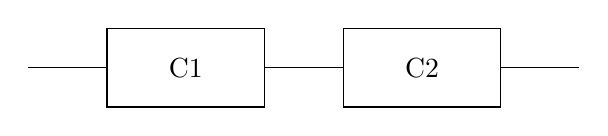
\begin{tikzpicture}[node distance=2cm]
                \node[coordinate, name=input] {};
                \node[
                    draw,
                    minimum width=2cm,
                    minimum height=1cm,
                    right of=input
                ] (c1) {C1};
                \node[
                    draw,
                    minimum width=2cm,
                    minimum height=1cm,
                    node distance=3cm,
                    right of=c1
                ] (c2) {C2};
                \node[coordinate, name=output, right of=c2] {};
                \draw[-] (input) -- (c1);
                \draw[-] (c1) -- (c2);
                \draw[-] (c2) -- (output);
            \end{tikzpicture}
        \end{center}
        \item \important{Parallel}: The system can work as long as at least one component works.
        \begin{center}
            \begin{tikzpicture}[node distance=2cm]
                \draw (0,0) -- (1,0);

                \draw (1,0) -- (1,1);
                \draw (1,0) -- (1,-1);

                \draw (1,1) -- (2,1);
                \draw (1,-1) -- (2,-1);

                \node[
                    draw,
                    minimum width=2cm,
                    minimum height=1cm,
                    name=c1
                ] at (3,1) {C1};
                \node[
                    draw,
                    minimum width=2cm,
                    minimum height=1cm,
                    name=c2
                ] at (3,-1) {C2};

                \draw (c1) -- (5,1);
                \draw (c2) -- (5,-1);

                \draw (5,1) -- (5,0);
                \draw (5,-1) -- (5,0);

                \draw (5,0) -- (6,0);
            \end{tikzpicture}
        \end{center}
    \end{itemize}
    \item \important{Model Topology}: The RBD structure \textbf{may not match the physical system layout}, as it's focused on \emph{functional success paths} rather than actual wiring or data flow.
\end{itemize}
Every element in the RBD has its \textbf{own reliability}. Blocks are combined together to model all possible success paths.

\highspace
\begin{flushleft}
    \textcolor{Green3}{\faIcon{square-root-alt} \textbf{Mathematical Concepts}}
\end{flushleft}
\begin{itemize}
    \item \important{Series Configuration}. In a \textbf{series system}, \textbf{all components must work} for the system to function. If \textbf{any single component fails}, the \textbf{whole system fails}. In other words, the system failure is determined by the failure of the \emph{first} component.

    The formula is:
    \begin{equation}
        R_S(t) = R_{C1}(t) \cdot R_{C2}(t) \cdot \dots \cdot R_{Cn}(t) = \prod_{i=1}^{n} R_i(t)
    \end{equation}
    Where:
    \begin{itemize}
        \item $R_S(t)$: system reliability at time $t$.
        \item $R_i(t)$: reliability of the $i^\text{th}$ component.
        \item This assumes \textbf{independent} component failures.
    \end{itemize}
    If each component has a \textbf{probability} $R_i(t)$ of working, then the \textbf{joint probability} that \textbf{all work} is the \textbf{product}.

    \begin{examplebox}[: Series Configuration]
        Consider, for example, the following model:
        \begin{center}
            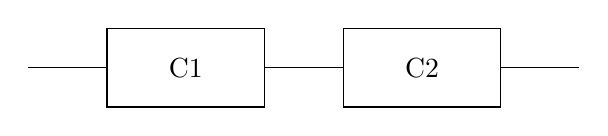
\begin{tikzpicture}[node distance=2cm]
                \node[coordinate, name=input] {};
                \node[
                    draw,
                    minimum width=2cm,
                    minimum height=1cm,
                    right of=input
                ] (c1) {C1};
                \node[
                    draw,
                    minimum width=2cm,
                    minimum height=1cm,
                    node distance=3cm,
                    right of=c1
                ] (c2) {C2};
                \node[coordinate, name=output, right of=c2] {};
                \draw[-] (input) -- (c1);
                \draw[-] (c1) -- (c2);
                \draw[-] (c2) -- (output);
            \end{tikzpicture}
        \end{center}
        The reliability is: $R_{S}(t) = R_{C1}(t) \cdot R_{C2}(t)$.
    \end{examplebox}


    \item \important{Parallel Configuration}. In a \textbf{parallel system}, the system functions as long as \textbf{at least one component works}. This configuration is used for \textbf{redundancy}. In other words, the system fails when the \emph{last} component fails.

    The formula is:
    \begin{equation}
        R_S(t) = 1 - \displaystyle\prod_{i=1}^{n} \left[1 - R_i(t)\right]
    \end{equation}
    Where:
    \begin{itemize}[label=*]
        \item $1 - R_i(t)$: failure probability of component $i$.
        \item $\displaystyle\prod_{i=1}^{n} \left[1 - R_i(t)\right]$: probability that \textbf{all fail}.
        \item $1 - \text{(all fail)}$: probability that \textbf{at least one works}.
    \end{itemize}
    In summary, the system works in a parallel configuration \textbf{as long as at least one component is functioning}. This \textbf{design increases fault tolerance and improves reliability}.

    \begin{examplebox}[: Parallel Configuration]
        Consider, for example, the following model:
        \begin{center}
            \begin{tikzpicture}[node distance=2cm]
                \draw (0,0) -- (1,0);

                \draw (1,0) -- (1,1);
                \draw (1,0) -- (1,-1);

                \draw (1,1) -- (2,1);
                \draw (1,-1) -- (2,-1);

                \node[
                    draw,
                    minimum width=2cm,
                    minimum height=1cm,
                    name=c1
                ] at (3,1) {C1};
                \node[
                    draw,
                    minimum width=2cm,
                    minimum height=1cm,
                    name=c2
                ] at (3,-1) {C2};

                \draw (c1) -- (5,1);
                \draw (c2) -- (5,-1);

                \draw (5,1) -- (5,0);
                \draw (5,-1) -- (5,0);

                \draw (5,0) -- (6,0);
            \end{tikzpicture}
        \end{center}
        The reliability is: $R_S(t) = R_{C1}(t) + R_{C2}(t) - R_{C1}(t) \cdot R_{C2}(t)$.
    \end{examplebox}
\end{itemize}

\newpage

\begin{flushleft}
    \textcolor{Green3}{\faIcon{book} \textbf{Other Series Formulas Related to Reliability}}
\end{flushleft}
\begin{itemize}
    \item \definition{Reliability Function of Series Systems as one Exponential Component $\lambda_{S}$}. In a \textbf{series system}, all components must function for the system to work. If one fails, the system fails. For $n$ components with exponential reliability:
    \begin{equation}
        R_S(t) = \displaystyle\prod_{i=1}^{n} R_i(t) = \displaystyle\prod_{i=1}^{n} e^{-\lambda_i t} = \exp\left(-t \displaystyle \sum_{i=1}^n \lambda_i\right)
    \end{equation}
    We define:
    \begin{equation}
        \lambda_S = \sum_{i=1}^n \lambda_i \quad \Longrightarrow \quad R_S(t) = e^{-\lambda_S t}
    \end{equation}
    This models the \textbf{system as one exponential component} with rate $\lambda_S$.


    \item \definition{Failure in Time (FIT)}. The \textbf{failure rate} of the whole system in series is:
    \begin{equation}
        \lambda_S = \displaystyle\sum_{i=1}^{n} \lambda_i
    \end{equation}
    This tells us that \textbf{each new component added in series increases the failure rate}, reducing overall reliability.


    \item \definition{Mean Time To Failure (MTTF)}. For an exponential distribution:
    \begin{equation}
        \text{MTTF}_{S} = \dfrac{1}{\lambda_{S}} = \dfrac{1}{\displaystyle\sum_{i=1}^{n} \lambda_{i}} = \dfrac{1}{\displaystyle\sum_{i=1}^{n} \dfrac{1}{\text{MTTF}_{i}}}
    \end{equation}
    Thus, the more components in series, the lower the systems's MTTF. If even one component is fragile, it significantly impacts the whole system.


    \item \important{Special Case: Identical Components}. Assume $n$ components and \textbf{same failure rate} $\lambda$, then:
    \begin{equation}
        \lambda_{S} = n \cdot \lambda \quad \Longrightarrow \quad R_{S}(t) = e^{-n \lambda t}
    \end{equation}
    And:
    \begin{equation}
        \text{MTTF}_{S} = \dfrac{1}{n \cdot \lambda}
    \end{equation}
    System becomes $n$ \textbf{time less reliable} than a single component.

    \item \definition{Availability of Series System}. Let $A_i = \frac{\text{MTTF}_i}{\text{MTTF}_i + \text{MTTR}_i}$ as the availability of component $i$, then:
    \begin{equation}
        A_S = \displaystyle\prod_{i=1}^{n} A_i
    \end{equation}
    And \hl{if all components are identical}:
    \begin{equation*}
        A_S = A^{n}
    \end{equation*}
    Where:
    \begin{equation*}
        A = \left(\dfrac{\text{MTTF}}{\text{MTTF} + \text{MTTR}}\right)^{n}
    \end{equation*}
    As with reliability, \textbf{availability degrades multiplicatively} in series configurations.
\end{itemize}

\newpage

\begin{flushleft}
    \textcolor{Green3}{\faIcon{book} \textbf{Other Parallel Formulas Related to Reliability}}
\end{flushleft}
\begin{itemize}
    \item \definition{Reliability Function of Parallel Systems}. Let $R_{i}(t)$ be the reliability of component $i$. Then the system reliability is:
    \begin{equation*}
        R_S(t) = 1 - \displaystyle\prod_{i=1}^{n} \left[1 - R_i(t)\right]
    \end{equation*}
    \begin{itemize}
        \item $1 - R_i(t)$: probability that component $i$ has failed by time $t$.
        \item $\prod (1 - R_i(t))$: probability that \textbf{all components} have failed.
        \item So, $1 - \text{(all failed)}$: probability that \textbf{at least one} is working.
    \end{itemize}


    \item \important{Special Case: Identical Components}. If all $n$ components have the \textbf{same reliability} $R(t)$, then:
    \begin{equation}
        R_S(t) = 1 - \left(1 - R\left(t\right)\right)^{n}
    \end{equation}
    As $n$ increases, $R_S(t) \to 1$: very high system reliability.


    \item \definition{Mean Time To Failure (MTTF)}. For parallel systems with exponential reliabilities $R_i(t) = e^{-\lambda_{i} t}$, there is \textbf{no simple closed-form MTTF} in the general case, but for identical components, if $R(t) = e^{-\lambda t}$, then:
    \begin{equation}
        R_S(t) = 1 - \left(1 - e^{-\lambda t}\right)^{n}
    \end{equation}
    MTTF can be found via integration:
    \begin{equation}
        \text{MTTF}_S = \displaystyle\int_{0}^{\infty} R_S(t) \, \mathrm{d}t
    \end{equation}
    This yields increasingly large values as $n$ increases (more redundancy, then more robust).


    \item \definition{Availability of Parallel System}. Let $A_i$ be the availability of component $i$, then:
    \begin{equation}
        A_{S} = 1 - \displaystyle\prod_{i=1}^n \left(1 - A_{i}\right)
    \end{equation}
    \hl{If all components are the same}:
    \begin{equation}
        A_{S} = 1 - \left(1 - A\right)^{n}
    \end{equation}
    Where:
    \begin{equation}
        A = \frac{\text{MTTF}}{\text{MTTF} + \text{MTTR}}
    \end{equation}
\end{itemize}

\begin{figure}[!htp]
    \centering
    \includegraphics[width=\textwidth]{img/reliability.pdf}
    \captionsetup{singlelinecheck=off}
    \caption[]{The \textbf{left plot} shows the series system reliability:
    \begin{itemize}
        \item Each line corresponds to a system composed of $n = 1, 2, 3, 4$ components in \textbf{series}.
        \item The $x$-axis is time (0 to 1000 hours).
        \item The $y$-axis is the system reliability $R_{S}(t)$, which \textbf{decreases over time}.
    \end{itemize}
    For $n=1$, the system is just a single component, standard exponential decay. As $n$ increases, reliability drops \textbf{faster} because the \textbf{probability of at least one failure increases}. Mathematically:
    \begin{equation*}
        R_S(t) = e^{-n \lambda t}
    \end{equation*}
    For example, with $n=4$, the system becomes much less reliable in shorter timeframes. This means that series systems are fragile; the more components there are, the greater the chance of failure. It's like a chain: the system is only as strong as its weakest link.
    
    The \textbf{right plot} shows the parallel system reliability:
    \begin{itemize}
        \item Each curve is a system with $n = 1$ to $n = 4$ components in \textbf{parallel}.
        \item The \textbf{system works as long as at least one component works}.
    \end{itemize}
    For $n=1$, it's the same as the single-component series case. As $n$ increases, reliability increases and curves stay higher for longer. Formula used:
    \begin{equation*}
        R_S(t) = 1 - \left(1 - e^{-\lambda t}\right)^{n}
    \end{equation*}
    The system becomes more fault-tolerant because it tolerates some component failures. This means that parallelism boosts reliability. With just 3 or 4 redundant units, reliability stays close to 1 for long durations.}
\end{figure}


\newpage\newpage\newpage\newpage\newpage\newpage\newpage\newpage

\begin{flushleft}
    \textcolor{Green3}{\faIcon{bookmark} \textbf{A quick recap}}
\end{flushleft}
\begin{itemize}
    \item \important{Series}
    \begin{center}
        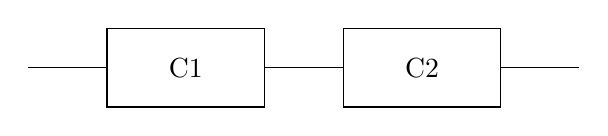
\begin{tikzpicture}[node distance=2cm]
            \node[coordinate, name=input] {};
            \node[
                draw,
                minimum width=2cm,
                minimum height=1cm,
                right of=input
            ] (c1) {C1};
            \node[
                draw,
                minimum width=2cm,
                minimum height=1cm,
                node distance=3cm,
                right of=c1
            ] (c2) {C2};
            \node[coordinate, name=output, right of=c2] {};
            \draw[-] (input) -- (c1);
            \draw[-] (c1) -- (c2);
            \draw[-] (c2) -- (output);
        \end{tikzpicture}
    \end{center}

    Reliability:
    \begin{equation*}
        R_{s} = \displaystyle\prod_{i}^{n} R_{i} \Longrightarrow R_{s} = R_{C1} \cdot R_{C2}
    \end{equation*}
    

    \item \important{Parallel}
    \begin{center}
        \begin{tikzpicture}[node distance=2cm]
            \draw (0,0) -- (1,0);

            \draw (1,0) -- (1,1);
            \draw (1,0) -- (1,-1);

            \draw (1,1) -- (2,1);
            \draw (1,-1) -- (2,-1);

            \node[
                draw,
                minimum width=2cm,
                minimum height=1cm,
                name=c1
            ] at (3,1) {C1};
            \node[
                draw,
                minimum width=2cm,
                minimum height=1cm,
                name=c2
            ] at (3,-1) {C2};

            \draw (c1) -- (5,1);
            \draw (c2) -- (5,-1);

            \draw (5,1) -- (5,0);
            \draw (5,-1) -- (5,0);

            \draw (5,0) -- (6,0);
        \end{tikzpicture}
    \end{center}

    Reliability:
    \begin{equation*}
        R_S(t) = R_{C1}(t) + R_{C2}(t) - R_{C1}(t) \cdot R_{C2}(t)
    \end{equation*}


    \item \important{Series-Parallel} (\textbf{Component Redundancy})
    \begin{center}
        \begin{tikzpicture}[node distance=2cm]
            \draw (0,0) -- (1,0);

            \draw (1,0) -- (1,1);
            \draw (1,0) -- (1,-1);

            \draw (1,1) -- (2,1);
            \draw (1,-1) -- (2,-1);

            \node[
                draw,
                minimum width=2cm,
                minimum height=1cm,
                name=c1
            ] at (3,1) {C1};
            \node[
                draw,
                minimum width=2cm,
                minimum height=1cm,
                name=c2
            ] at (3,-1) {C2};

            \draw (c1) -- (5,1);
            \draw (c2) -- (5,-1);

            \draw (5,1) -- (5,0);
            \draw (5,-1) -- (5,0);

            \draw (5,0) -- (6,0);

            \draw (6,0) -- (6,1);
            \draw (6,0) -- (6,-1);

            \draw (6,1) -- (7,1);
            \draw (6,-1) -- (7,-1);

            \node[
                draw,
                minimum width=2cm,
                minimum height=1cm,
                name=c3
            ] at (8,1) {C3};
            \node[
                draw,
                minimum width=2cm,
                minimum height=1cm,
                name=c4
            ] at (8,-1) {C4};

            \draw (c3) -- (10,1);
            \draw (c4) -- (10,-1);

            \draw (10,1) -- (10,0);
            \draw (10,-1) -- (10,0);

            \draw (10,0) -- (11,0);
        \end{tikzpicture}
    \end{center}

    Reliability:
    \begin{equation*}
        R_{S}(t) = \left(R_{C1} + R_{C2} - R_{C1} \cdot R_{C2}\right) \cdot \left(R_{C3} + R_{C4} - R_{C3} \cdot R_{C4}\right)
    \end{equation*}


    \item \important{Parallel-Series} (\textbf{System Redundancy})
    \begin{center}
        \begin{tikzpicture}[node distance=2cm]
            \draw (0,0) -- (1,0);

            \draw (1,0) -- (1,1);
            \draw (1,0) -- (1,-1);

            \draw (1,1) -- (2,1);
            \draw (1,-1) -- (2,-1);

            \node[
                draw,
                minimum width=2cm,
                minimum height=1cm,
                name=c1
            ] at (3,1) {C1};
            \node[
                draw,
                minimum width=2cm,
                minimum height=1cm,
                name=c2
            ] at (3,-1) {C2};

            \draw (c1) -- (6,1);
            \draw (c2) -- (6,-1);

            \node[
                draw,
                minimum width=2cm,
                minimum height=1cm,
                name=c3
            ] at (7,1) {C3};
            \node[
                draw,
                minimum width=2cm,
                minimum height=1cm,
                name=c4
            ] at (7,-1) {C4};

            \draw (c3) -- (9,1);
            \draw (c4) -- (9,-1);

            \draw (9,1) -- (9,0);
            \draw (9,-1) -- (9,0);

            \draw (9,0) -- (10,0);
        \end{tikzpicture}
    \end{center}

    Reliability:
    \begin{equation*}
        R_{s} = 1 - \left[\left(1 - R_{C1} \cdot R_{C3}\right) \cdot \left(1 - R_{C2} \cdot R_{C4}\right)\right]
    \end{equation*}
\end{itemize}

\newpage

\begin{examplebox}[: calculate the reliability of the system]
    \begin{flushleft}
        \textcolor{Green3}{\faIcon{question-circle} \textbf{Question}}
    \end{flushleft}
    What is the Reliability of the entire system knowing the reliability of each component?
    \begin{center}
        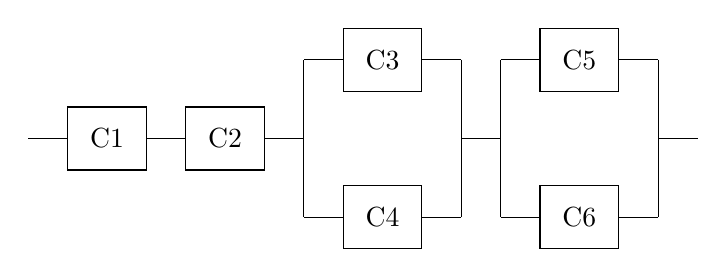
\begin{tikzpicture}[node distance=1cm]
            \draw (0,0) -- (0.5,0);

            \node[
                draw,
                minimum width=1cm,
                minimum height=.8cm,
                name=c1
            ] at (1,0) {C1};

            \draw (1.5,0) -- (2,0);

            \node[
                draw,
                minimum width=1cm,
                minimum height=.8cm,
                name=c2
            ] at (2.5,0) {C2};

            \draw (3,0) -- (3.5,0);

            \draw (3.5,0) -- (3.5,1);
            \draw (3.5,0) -- (3.5,-1);

            \draw (3.5,1) -- (4,1);
            \draw (3.5,-1) -- (4,-1);

            \node[
                draw,
                minimum width=1cm,
                minimum height=.8cm,
                name=c3
            ] at (4.5,1) {C3};
            \node[
                draw,
                minimum width=1cm,
                minimum height=.8cm,
                name=c4
            ] at (4.5,-1) {C4};

            \draw (5,1) -- (5.5,1);
            \draw (5,-1) -- (5.5,-1);

            \draw (5.5,1) -- (5.5,0);
            \draw (5.5,-1) -- (5.5,0);

            \draw (5.5,0) -- (6,0);

            \draw (6,0) -- (6,1);
            \draw (6,0) -- (6,-1);

            \draw (6,1) -- (6.5, 1);
            \draw (6,-1) -- (6.5, -1);

            \node[
                draw,
                minimum width=1cm,
                minimum height=.8cm,
                name=c5
            ] at (7,1) {C5};
            \node[
                draw,
                minimum width=1cm,
                minimum height=.8cm,
                name=c6
            ] at (7,-1) {C6};

            \draw (7.5,1) -- (8, 1);
            \draw (7.5,-1) -- (8, -1);

            \draw (8,1) -- (8,0);
            \draw (8,-1) -- (8,0);

            \draw (8,0) -- (8.5,0);
        \end{tikzpicture}
    \end{center}
    \begin{multicols}{3}
        \begin{itemize}
            \item $R_{C1} = 0.95$
            \item $R_{C2} = 0.97$
            \item $R_{C3} = 0.99$
            \item $R_{C4} = 0.99$
            \item $R_{C5} = 0.92$
            \item $R_{C6} = 0.92$
        \end{itemize}
    \end{multicols}
    \begin{flushleft}
        \textcolor{Green3}{\faIcon{check} \textbf{Solution}}
    \end{flushleft}
    \begin{enumerate}
        \item Consider components $C1$ and $C2$. The reliability, which we will call $R_{G}$, is then calculated as a \emph{series}:
        \begin{equation*}
            R_{G} = R_{C1} \cdot R_{C2} = 0.95 \cdot 0.97 = 0.9215
        \end{equation*}

        \item Consider components $C3$ and $C4$. The reliability, which we will call $R_{H}$, is then calculated as a \emph{parallel}:
        \begin{equation*}
            \begin{array}{rcl}
                R_{H} &=& 1 - \left[\left(1-R_{C3}\right) \cdot \left(1-R_{C4}\right)\right] \\ [.5em]
                &=& 1 - \left[\left(1 - 0.99\right) \cdot \left(1 - 0.99\right)\right] \\ [.5em]
                &=& 1 - 0.0001 \\ [.5em]
                &=& 0.9999
            \end{array}
        \end{equation*}

        \item Consider components $C5$ and $C6$. The reliability, which we will call $R_{I}$, is then calculated as in the previous step:
        \begin{equation*}
            \begin{array}{rcl}
                R_{I} &=& 1 - \left[\left(1-R_{C5}\right) \cdot \left(1-R_{C6}\right)\right] \\ [.5em]
                &=& 1 - \left[\left(1 - 0.92\right) \cdot \left(1 - 0.92\right)\right] \\ [.5em]
                &=& 1 - 0.0064 \\ [.5em]
                &=& 0.9936
            \end{array}
        \end{equation*}

        \item Finally, we calculate the reliability of the system by multiplying each calculated component reliability:
        \begin{equation*}
            \begin{array}{rcl}
                R_{s} &=& R_{G} \cdot R_{H} \cdot R_{I} \\ [.5em]
                &=& 0.9215 \cdot 0.9999 \cdot 0.9936 \\ [.5em]
                &=& 0.91551083976 \approx 0.9155
            \end{array}
        \end{equation*}
    \end{enumerate}
\end{examplebox}

\begin{examplebox}[: calculate reliability without numbers]
    \begin{flushleft}
        \textcolor{Green3}{\faIcon{question-circle} \textbf{Question}}
    \end{flushleft}
    The system consists of 2 control blocks and 3 voice channels. The system is up when at least 1 control channel and at least 1 voice channel are up.
    \begin{center}
        \includegraphics[width=\textwidth]{img/RBD-6.pdf}
    \end{center}
    \begin{flushleft}
        \textcolor{Green3}{\faIcon{check} \textbf{Solution}}
    \end{flushleft}
    Reliability can be calculated in parallel, as it takes almost a component to work properly. Each control channel has reliability $R_{c}$ and each voice channel has reliability $R_{v}$:
    \begin{equation*}
        R = \left[1 - \left(1 - R_{c}\right)^{2}\right] \cdot \left[1 - \left(1 - R_{v}\right)^{3}\right]
    \end{equation*}
\end{examplebox}

\newpage

\paragraph{R out of N redundancy (RooN)}

An \definition{RooN ($r$ out of $n$)} redundancy system \textbf{contains} both the \textbf{series system model and the parallel system model} as special cases. The system has $n$ components that operate or fail independently of one another and as long as at least $r$ of these components (any $r$) survive, the system survives.\cite{nist8184Model}

\highspace
A system with:
\begin{itemize}
    \item $n$: total number of identical components.
    \item $r$: minimum number of components that must \textbf{work correctly}.
\end{itemize}
The system function \textbf{if at least $r$ out of the $n$ components are operational}. \textbf{System failure occurs when} the $\left(n - r + 1\right)$-th component failure occurs.\cite{nist8184Model}

\highspace
But note an interesting observation:
\begin{itemize}
    \item When $r=n$, the $r$ out of $n$ model reduces to the \textbf{series} model.\cite{nist8184Model}
    \item When $r=1$, the $r$ out of $n$ model becomes the \textbf{parallel} model.\cite{nist8184Model}
\end{itemize}
In simple terms, \texttt{RooN} is a system made up of $n$ identical replicas, where at least $r$ replicas have to work well for the whole system to work well.

\highspace
The reliability formula for the RooN system is:
\begin{equation}
	R_{s}\left(t\right) = R_{V} \displaystyle\sum_{i=r}^{n} R_{c}^{i} \left(1 - R_{c}\right)^{n-i} \: \dfrac{n!}{i!\left(n-i\right)!}
\end{equation}
Where:
\begin{itemize}
    \item $n$: total number of identical components.
    \item $R_c(t)$: reliability of each component.
    \item $R_V(t)$: reliability of the \textbf{voter} (which combines outputs).
    \item $R_S(t)$: system reliability.
    \item $\left(1 - R_{c}\right)^{n-i}$: failure probability of the remaining $n-i$.
\end{itemize}
\begin{figure}[!htp]
	\centering
	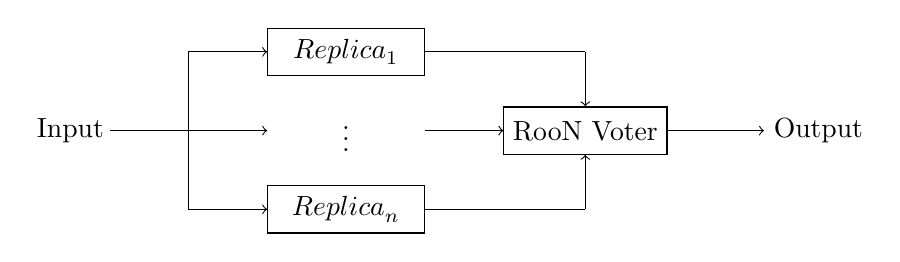
\begin{tikzpicture}[node distance=2cm]
        \node[rectangle, name=input] at (-0.5,0) {Input};

        \draw (0,0) -- (1,0);

        \draw (1,0) -- (1,1);
        \draw (1,0) -- (1,-1);
        \draw[->] (1,0) -- (2,0);

        \draw[->] (1,1) -- (2,1);
        \draw[->] (1,-1) -- (2,-1);

        \node[
            draw,
            minimum width=2cm,
            minimum height=0.6cm,
            name=replica1
        ] at (3,1) {$\text{Replica}_{1}$};
        \node[
            rectangle,
            minimum width=2cm,
            minimum height=0.6cm,
            name=replicaDots
        ] at (3,0) {$\vdots$};
        \node[
            draw,
            minimum width=2cm,
            minimum height=0.6cm,
            name=replicaN
        ] at (3,-1) {$\text{Replica}_{n}$};

        \draw (replica1) -- (6.04,1);
        \draw[->] (replicaDots) -- (5,0);
        \draw (replicaN) -- (6.04,-1);

        \node[
            draw,
            minimum width=2cm,
            minimum height=0.6cm,
            name=roonVoter
        ] at (6.04,0) {RooN Voter};

        \draw[->] (6.04,1) -- (roonVoter);
        \draw[->] (6.04,-1) -- (roonVoter);

        \node[rectangle, name=output] at (9,0) {Output};

        \draw[->] (roonVoter) -- (output);
    \end{tikzpicture}
	\caption{General structure of RooN system.}
\end{figure}

\noindent
The reliability of the \textbf{central voter} $R_{V}(t)$ is crucial. If the voter fails, the system fails, even if enough components are still working. In practice, voter reliability is either assumed perfect $\left(R_{V} = 1\right)$ or modeled separately.

\newpage

\paragraph{Triple Modular Redundancy (TMR)}

\definition{Triple Modular Redundancy (TMR)} is a fault-tolerant form of N-modular redundancy, in which \textbf{three systems perform a process and the result is processed by a majority-voting system to produce a single output}. If any \textbf{one of the three systems fails}, the \textbf{other two systems can correct and mask the fault}.

\highspace
The system works properly if 2 out of 3 components work properly \textbf{\underline{and}} the voter works properly.

\highspace
The \definition{TMR Reliability $R_{TMR}$} is:
\begin{equation}
	R_{TMR} = R_{v}\left(3 \cdot R_{m}^{2} - 2 \cdot R_{m}^{3}\right)
\end{equation}
And the \definition{TMR MTTF $MTTF_{TMR}$} is:
\begin{equation}
	\texttt{MTTF}_{TMR} = \dfrac{5}{6} \cdot MTTF_{\text{simplex}}
\end{equation}

\begin{flushleft}
	\textcolor{Green3}{\faIcon{question-circle} \textbf{TMR: good or bad?}}
\end{flushleft}
TMR systems can \textbf{tolerate} both \textbf{transient}\footnote{In electrical engineering, a \definition{transient fault} is defined as an error condition that vanishes after the power is disconnected and restored.} \textbf{and permanent faults}\footnote{In electrical engineering, a persistent or \definition{permanent faults} are a type of fault that is present regardless of the disconnection of the power supply.}. It also has \textbf{higher reliability} (for shorter missions).

\highspace
The \textbf{TMR reliability} can be the \textbf{same as the series systems} if:
\begin{equation}
	R_{TMR}\left(t\right) = R_{c}\left(t\right) \Longrightarrow 3e^{-2 \lambda_{m} t} - 2e^{-3 \lambda_{m} t} = e^{-\lambda_{m} t}
\end{equation}
The time $t$ is:
\begin{equation}
	t = \dfrac{\ln\left(2\right)}{\lambda_{m}} \approx 0.7 \: \texttt{MMTF}_{c}
\end{equation}
Note that $R_{TMR}\left(t\right) > R_{c}\left(t\right)$ when mission time is less than 70\% of $\texttt{MTTF}_{c}$.

\newpage

\paragraph{Standby redundancy}

\definition{Standby redundancy} is a system consisting of two parallel replicas:
\begin{itemize}
	\item The \emph{primary} replica, which \textbf{operates all the time}.
	\item The \emph{redundant} replica (generally disabled) is \textbf{activated when the primary replica fails}.
\end{itemize}
\begin{figure}[!htp]
	\centering
	\includegraphics[width=.6\textwidth]{img/standby-redundancy-1.pdf}
\end{figure}

\noindent
\textbf{To be operational}, the standby system requires two mechanisms:
\begin{enumerate}
	\item A mechanism to \textbf{determine whether or not the primary replica is functioning properly} (on-line self check);
	\item A dynamic switching mechanism to \textbf{deactivate the primary replica and activate the redundant replica}.
\end{enumerate}

\begin{table}[!htp]
	\centering
	\begin{tabular}{@{} p{13em} | p{18em} @{}}
		\toprule
		\textbf{Standby Parallel Model} & \textbf{System Reliability} \\
		\midrule
		Equal failure rates, perfect switching & $R_{s} = e^{-\lambda t}\left(1 + \lambda t\right)$ \\
		Unequal failure rates, perfect switching & $R_{s} = e^{-\lambda_{1} t} + \lambda_{1} \dfrac{\left(e^{-\lambda_{1} t} - e^{-\lambda_{2} t}\right)}{\lambda_{2}-\lambda_{1}}$ \\
		Equal failure rates, imperfect switching & $R_{s} = e^{-\lambda t} \left(1 + R_{\text{switch}} \lambda t\right)$ \\
		Unequal failure rates, imperfect switching & $R_{s} = e^{-\lambda_{1} t} + R_{\text{switch}}\lambda_{1} \dfrac{\left(e^{-\lambda_{1} t} - e^{-\lambda_{2} t}\right)}{\lambda_{2} - \lambda_{1}}$ \\
		\bottomrule
	\end{tabular}
	\caption{Standby redundancy - Quick Formulas.}
\end{table}

\noindent
In the previous table we have:
\begin{itemize}
	\item $R_{s}$: System Reliability
	\item $\lambda$: Failure Rate
	\item $t$: Operating Time
	\item $R_{\text{switch}}$: Switching Reliability
\end{itemize}